\definecolor{statblue}{HTML}{2E75A8}
\definecolor{statorange}{HTML}{D77819}
\definecolor{statpurple}{HTML}{7654A3}
\definecolor{statteal}{HTML}{267A68}
\definecolor{statgray}{HTML}{A9B4BE}

\newcommand{\timepanel}{%
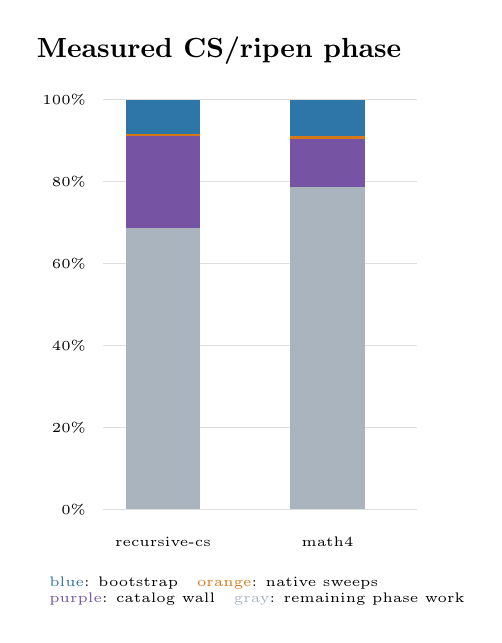
\begin{tikzpicture}[x=0.95cm,y=0.052cm,font=\footnotesize]
\node[font=\bfseries] at (2.4,112) {Measured CS/ripen phase};
\foreach \tick in {0,20,40,60,80,100}{%
  \node[font=\tiny,anchor=east] at (0.75,\tick) {\tick\%};
  \draw[gray!25] (0.85,\tick) -- (5.05,\tick);
}
\fill[statgray] (1.15,0) rectangle (2.15,68.73);
\fill[statpurple] (1.15,68.73) rectangle (2.15,91.07);
\fill[statorange] (1.15,91.07) rectangle (2.15,91.57);
\fill[statblue] (1.15,91.57) rectangle (2.15,100);
\fill[statgray] (3.35,0) rectangle (4.35,78.65);
\fill[statpurple] (3.35,78.65) rectangle (4.35,90.34);
\fill[statorange] (3.35,90.34) rectangle (4.35,91.08);
\fill[statblue] (3.35,91.08) rectangle (4.35,100);
\node[font=\tiny,align=center] at (1.65,-8) {recursive-cs};
\node[font=\tiny,align=center] at (3.85,-8) {math4};
\node[font=\tiny,align=left,anchor=west] at (0,-20) {\textcolor{statblue}{blue}: bootstrap\quad\textcolor{statorange}{orange}: native sweeps\\
\textcolor{statpurple}{purple}: catalog wall\quad\textcolor{statgray}{gray}: remaining phase work};
\end{tikzpicture}}

\newcommand{\queuepanel}{%
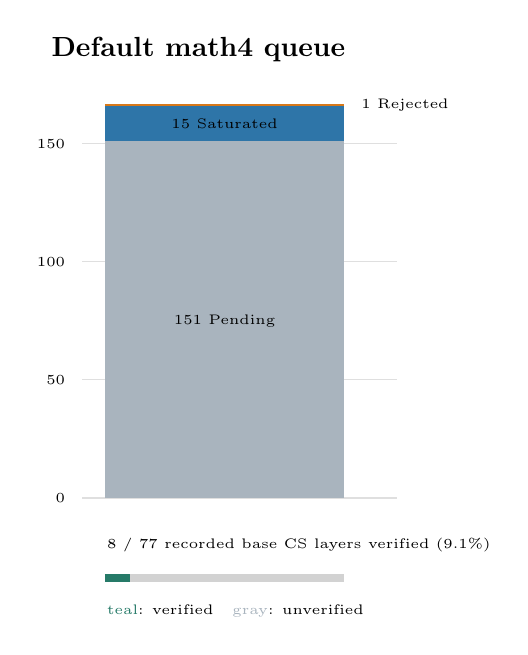
\begin{tikzpicture}[x=0.95cm,y=0.030cm,font=\footnotesize]
\node[font=\bfseries] at (2.4,190) {Default math4 queue};
\foreach \tick in {0,50,100,150}{%
  \node[font=\tiny,anchor=east] at (0.75,\tick) {\tick};
  \draw[gray!25] (0.85,\tick) -- (5.05,\tick);
}
\fill[statgray] (1.15,0) rectangle (4.35,151);
\fill[statblue] (1.15,151) rectangle (4.35,166);
\fill[statorange] (1.15,166) rectangle (4.35,167);
\node[font=\tiny] at (2.75,75) {151 Pending};
\node[font=\tiny] at (2.75,158.5) {15 Saturated};
\node[font=\tiny,anchor=west] at (4.45,166.5) {1 Rejected};
\node[font=\tiny,anchor=west] at (1.05,-20) {8 / 77 recorded base CS layers verified (9.1\%)};
\draw[statteal,line width=3pt] (1.15,-34) -- (1.15+3.2*8/77,-34);
\draw[gray!35,line width=3pt] (1.15+3.2*8/77,-34) -- (4.35,-34);
\node[font=\tiny,anchor=west] at (1.05,-48) {\textcolor{statteal}{teal}: verified\quad\textcolor{statgray}{gray}: unverified};
\end{tikzpicture}}

\newcommand{\StatsFigure}{%
\begin{figure}[t]\centering
\begin{minipage}[t]{.49\linewidth}\centering\timepanel\end{minipage}\hfill
\begin{minipage}[t]{.49\linewidth}\centering\queuepanel\end{minipage}
\caption{Recent bounded native observations. The left panel uses disjoint portions
of the measured phase from five-run medians: bootstrap, native sweeps, catalog wall,
and remaining phase work. Catalog wall includes catalog I/O and grouping; exact graph
comparison alone was 0.58\% of recursive-cs and 1.08\% of math4. The right panel is
the default four-round math4 queue: 15 Saturated, 1 Rejected, and 151 Pending
candidates, with 8 of 77 recorded base CS layers verified. These are bounded
experiments; Pending is not a negative result, and the coverage denominator is the
recorded base-CS population, not every possible layer or the live tier0 graph.}
\label{fig:stats}
\end{figure}}
